% Fig. 1: stages of the monitoring pipeline, one journal column (83.5 mm) wide.
\documentclass[border=0.5pt]{standalone}
\usepackage{newtxtext}
\usepackage{tikz}
\usetikzlibrary{arrows.meta}
\begin{document}
\fontsize{8}{9.4}\selectfont
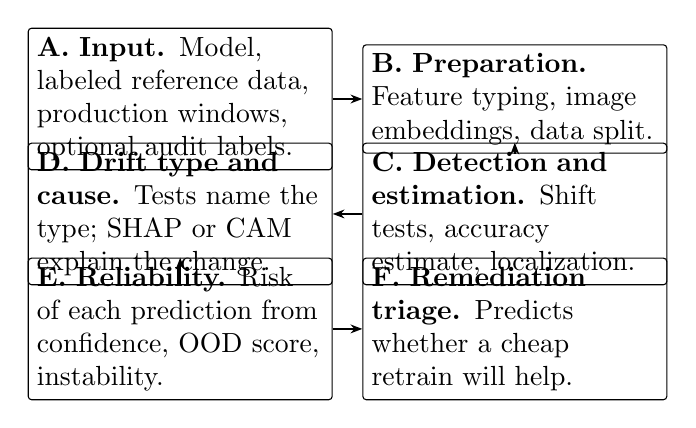
\begin{tikzpicture}[
  stage/.style={draw, rounded corners=1.2pt, text width=36.4mm, minimum height=11.6mm, inner sep=1.1mm,
                align=left, execute at begin node={\hyphenpenalty=10000\rightskip=0pt plus 1fil}},
  flow/.style={-{Stealth[length=1.5mm]}, semithick}]
\node[stage] (A) at (0,0)        {\textbf{A. Input.} Model, labeled reference data, production windows, optional audit labels.};
\node[stage] (B) at (42.5mm,0)   {\textbf{B. Preparation.} Feature typing, image embeddings, data split.};
\node[stage] (C) at (42.5mm,-14.6mm) {\textbf{C. Detection and estimation.} Shift tests, accuracy estimate, localization.};
\node[stage] (D) at (0,-14.6mm)  {\textbf{D. Drift type and cause.} Tests name the type; SHAP or CAM explain the change.};
\node[stage] (E) at (0,-29.2mm)    {\textbf{E. Reliability.} Risk of each prediction from confidence, OOD score, instability.};
\node[stage] (F) at (42.5mm,-29.2mm) {\textbf{F. Remediation triage.} Predicts whether a cheap retrain will help.};
\draw[flow] (A) -- (B);
\draw[flow] (B) -- (C);
\draw[flow] (C) -- (D);
\draw[flow] (D) -- (E);
\draw[flow] (E) -- (F);
\end{tikzpicture}
\end{document}
